Theorem \ref{thm genRMT informal} characterizes the test error for learning using Lipschitz feature maps as a function of the three features population (cross-)covariances $\Omega, \Phi, \Psi$. For the particular case where both the target and learner feature maps are drawn from the Gaussian rainbow ensemble from~\Cref{def:rainbow}, these population covariances can be expressed in closed-form in terms of combinations of products of the weights matrices. Consider two rainbow networks
\begin{equation}
    \begin{split}
    \f(\x)&=\f_L(W_L\f_{L-1}(\dots \f_1(W_1 \x)))\\
     \fast(\x)&=\wt{\f}_{\wt{L}}(V_{\wt{L}} \wt{\f}_{\wt{L}-1}(\dots \wt{\f}_1(V_1 \x)))
     \end{split}
\end{equation}
with depths $L,\wt{L}$. The approach we introduce here is in theory capable of obtaining linear or polynomial approximations to $\Omega,\Phi,\Psi$ under very general assumptions. However, for definiteness we focus on a class of correlated rainbow networks in which we allow the $k$-th row of $W_\ell$ to be correlated only to the $k$-th row of $W_{\ell'},V_{\ell'}$ as this allows for particularly simple expressions for the linearized covariances\footnote{The identity matrices in~\Cref{eq lin cov} are a direct consequence of this assumption. In case of weight matrices with varying row-norms or covariances across rows the resulting expression would be considerably more complicated.}. Note that we explicitly allow for weights to be correlated across layers. 
\begin{assumption}[Correlated rainbow networks]\label{corr rainbow}
    By symmetry we assume without loss of generality $L\le \wt L$. Furthermore, for all \(\ell \leq L \leq \wt L\), we assume
    \begin{enumerate}[label=(\alph*)]
        \item All the internal widths $p_\ell$ of $W_\ell,V_\ell$ agree,
        \item The rows $w_\ell,v_\ell$ of $W_\ell,V_\ell$ are i.i.d. with mean zero and 
        \begin{equation*}
        C_\ell := p_\ell \E w_\ell w_\ell^\top, \; \wt C_\ell:=p_\ell\E v_\ell v_\ell^\top,\; \wc C_\ell:=p_\ell\E w_\ell v_\ell^\top,
        \end{equation*}
        with \(\norm{C_\ell} + \norm{\wt C_\ell} + \norm{\wc C_\ell}\lesssim 1\),
        \item Asymptotic orthogonality of the rows of \(W_\ell, V_\ell\). Let \(w, w'\) be two independent copies of a row of \(W_\ell\). Then, \(\braket{w, w'} \prec d^{-1/2}\), same for \(V_\ell\),
        \item The rows of \(W_\ell, V_\ell\) are sub-Gaussian random vectors: 
        \begin{equation}
            \norm{w_\ell}_{\psi_2} + \norm{v_\ell}_{\psi_2} = O(d^{-1/2}),
        \end{equation}
        \item Centered activation functions \(\f_\ell, \wt \f_\ell: \E_{\x} \f_{\ell}(W_{\ell} \f_{\ell - 1}(\ldots \f_1(W_1 \x))) = 0\), same for \(\wt \f_\ell\) (see~\Cref{ass:data+features}).
    \end{enumerate}
\end{assumption}
Under~\Cref{corr rainbow} the \emph{linearized population covariances} can be defined recursively as follows:
\begin{definition}[Linearized population covariances]
    \label{def: linearized_covs}
    Define the sequence of matrices $\Omega_\ell^\mathrm{lin},\Phi_\ell^\mathrm{lin}, \Psi_\ell^\mathrm{lin}$ by the recursions
    \begin{equation}\label{eq lin cov}
    \begin{split}
         & \Omega_{\ell}^{\mathrm{lin}}=(\kappa^1_\ell)^2 W_\ell\Omega_{\ell-1}^{\mathrm{lin}}W_\ell^\top+(\kappa^{*}_\ell)^2\mathbb{I}_{p_\ell}                             \\
         & \Psi_{\ell}^{\mathrm{lin}}=(\tilde{\kappa}^1_\ell )^2V_\ell\Psi_{\ell-1}^{\mathrm{lin}}V_\ell^\top+(\wt{\kappa}^{*}_\ell)^2\mathbb{I}_{p_\ell} \\
         & \Phi_{\ell}^{\mathrm{lin}}=\kappa^1_\ell\tilde{\kappa}^1_\ell W_\ell\Phi_{\ell-1}^{\mathrm{lin}} V_\ell^\top +(\wc{\kappa}^*_\ell)^2\mathbb{I}_{p_\ell},
         \end{split}
    \end{equation}
    with $\Omega_0^{\mathrm{lin}}=\Psi_0^{\mathrm{lin}}=\Phi_0^{\mathrm{lin}}=\Omega_0$ the input covariance.
    The coefficients $\{\kappa_\ell^1,\tilde{\kappa}_\ell^1,\kappa_\ell^*,\tilde{\kappa}_\ell^*, \wc{\kappa}^*_\ell\}$ are defined by the recursion
    \begin{equation}
        \kappa_\ell^1 := \E \f_\ell'(N_\ell), \quad \wt \kappa_\ell^1:=\E \wt\f_\ell'(\wt N_\ell)
    \end{equation}
    and 
    \begin{equation}
        \begin{split}
            \kappa^\ast_\ell &= \sqrt{\E[\f_\ell(N_\ell)^2]-r_\ell(\kappa^1_\ell)^2}                                         \\
            \tilde{\kappa}^*_\ell&= \sqrt{\E [\wt{\f}_\ell(\wt N_\ell)^2]-\tilde{r}_\ell(\tilde{\kappa}^1_\ell)^2} \\
            \wc{\kappa}^*_\ell&=\sqrt{\E [\f_\ell(N_\ell )\wt{\f}_\ell(\wt N_\ell)]-\check{r}_\ell \kappa^1_\ell\wt{\kappa}^1_\ell},
        \end{split}
    \end{equation}
    where $N_\ell,\wt N_\ell$ are jointly mean-zero Gaussian with $\E N_\ell^2=r_\ell$, $\E \wt N_\ell^2=\wt r_\ell$, $\E N_\ell\wt N_\ell=\wc r_\ell$, with 
    \begin{equation*}
        r_{\ell}=\Tr[C_\ell \Omega_{\ell-1}^{\mathrm{lin}}], \; \wt{r}_{\ell}=\Tr[\wt{C}_\ell \Psi_{\ell-1}^{\mathrm{lin}}],\; \wc{r}_{\ell}=\Tr[\wc{C}_\ell^\top \Phi_{\ell-1}^{\mathrm{lin}}].
    \end{equation*}
    Finally, for $\tilde{L}\ge \ell\ge L+1$, define
    \begin{equation}
    \begin{split}
         \Phi_{\ell}^{\mathrm{lin}}&=\wt{\kappa}^1_\ell \Phi_{\ell-1}^{\mathrm{lin}}V_\ell^\top,
         \end{split}
    \end{equation}
    with still $\wt\kappa_\ell^1,\wt\kappa_\ell^\ast$ just as before, and $ \Psi_{\ell}^{\mathrm{lin}}$ with the same recursion \eqref{eq lin cov}.
\end{definition}

\begin{conjecture}
    The populations covariances $\Omega, \Phi,\Psi$ involved in Theorem \ref{thm genRMT informal} can be asymptotically approximated with the last iterates of the linear recursions of Definition \ref{def: linearized_covs}, i.e.
    \begin{align}
        \norm{\Omega-\Omega_L^\mathrm{lin}}_F + \norm{\Psi-\Psi_{\tilde{L}}^\mathrm{lin}}_F + \norm{\Phi-\Phi_{\tilde{L}}^\mathrm{lin}}_F &\lesssim 1
    \end{align}
\end{conjecture}

Note that the linearization from~\Cref{def: linearized_covs} also provides good approximation to the population covariances $\Omega_\ell,\Phi_\ell,\Psi_\ell$ of the post-activations at intermediate layers $\ell$. The method we use to rigorously derive the linearizations is in theory applicable to any depths, however the estimates quickly become tedious. To keep the present work at a manageable length we provide a rigorous proof of concept only for the simplest multi-layer case.
\begin{theorem}\label{theo lin}
    Under~\Cref{corr rainbow} with $L=\wt L = 2$, we have 
    \begin{equation*}
        \begin{split}
        \norm{\Omega_1-\Omega_1^\mathrm{lin}}_F + \norm{\Psi_1-\Psi_1^\mathrm{lin}}_F + \norm{\Phi_1-\Phi_1^\mathrm{lin}}_F &\prec 1,\\
        \norm{\Omega_2 - \Omega_2^{\mathrm{lin}}}_F + 
        \norm{\Psi_2-\Psi_2^\mathrm{lin}}_F + \norm{\Phi_2-\Phi_2^\mathrm{lin}}_F&\prec 1.
        \end{split}
    \end{equation*} 
\end{theorem}
\begin{remark}[Comparison]
    The approach we take here is somewhat different from previous works~\cite{schroder2023deterministic,Fan2020SpectraOT,2306.05850} on (multi-layer) random feature models. In these previous results, the deterministic equivalent for the resolvent was obtained using primarily the randomness of the weights, resulting in relatively stringent assumptions (Gaussianity and independence between layers). This layer-by-layer recursive approach resulted in a deterministic equivalent for the resolvent which is \emph{consistent} with a sample covariance matrix with linearized population covariance. Here we take the direct approach of considering feature models with arbitrary structured features, and then linearize the population covariances in a separate step for random features.  
\end{remark}

\subsection{Proof of~\Cref{theo lin}}
    We sketch the main tools used in the argument and we refer the reader to~\cref{prop:lin_1_layer} and~\cref{thm:lin_app} for the formal proof.
    In the proof, we crucially rely on the theory of Wiener chaos expansion and Stein's method (see~\cite{nourdin2012normal}). Gaussian Wiener chaos is a generalization of Hermite polynomial expansions, which previously have been used for approximate linearization \cite{Fan2020SpectraOT,schroder2023deterministic} in similar contexts. The basic idea is to decompose random variables $F=F(\x)$ which are functions of the Gaussian random vector $\x$, into pairwise uncorrelated components 
    \begin{equation}
        F = \E F + \sum_{p\ge 1} I_p\Bigl(\frac{\E D^p F}{p!}\Bigr), 
    \end{equation}
    where $I_p$ is a so called \emph{multiple integral} (generalizing Hermite polynomials) and $D^p$ is the $p$-th Malliavin derivative. By applying this to the one-layer quantities $\f_1(w^\top \x),\f_1(u^\top \x)$ we obtain, for instance 
    \begin{equation}
    \begin{aligned}
        &\E \f_1(w^{\top} \x) \f_1(v^{\top} \x) \\
        &\quad = \sum_{p \geq 1} \frac{1}{p!} \E \f_1^{(p)}(w^\top \x) \E \f_1^{(p)}(u^\top \x) \braket{w, v}^p,
    \end{aligned}
    \end{equation}
    which for independent $w,v$ we can truncate after $p=1$, giving rise to the linearization. 
    
    For the multi-layer case we combine the chaos expansion with Stein's method in order to prove \emph{quantitative central limit theorems} of the type 
    \begin{equation}
        d_W(F,N) \lesssim \E \abs{\E F^2 - \braket{DF,-DL^{-1}F}}
    \end{equation}
    for the Wasserstein distance $d_W$, where
    \begin{equation}
        F := w^\top \phi_1(W\x),\quad  N\sim \mathcal N(0,\E F^2),
    \end{equation}
    and $L^{-1}$ is the pseudo-inverse of the \emph{generator of the Ornstein–Uhlenbeck semigroup}.  
    
    
\begin{figure}[t]
    \centering
    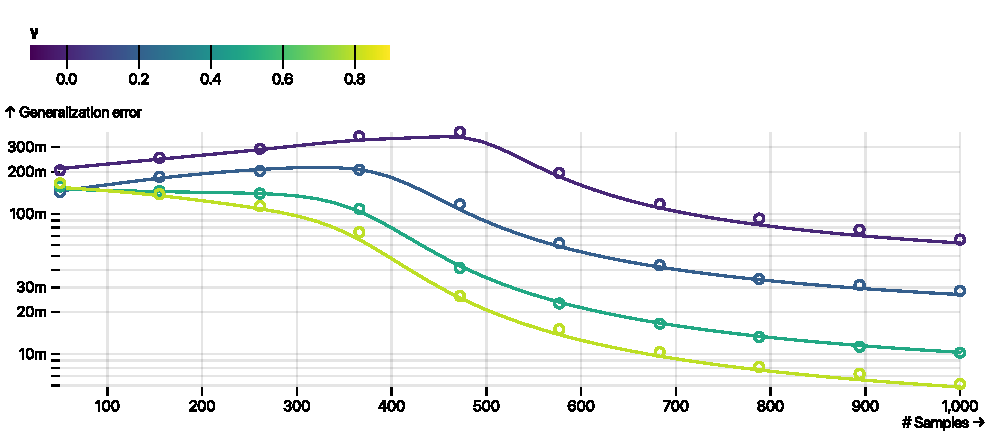
\includegraphics[scale=0.6]{chapters/deeprf/figs/rf_emp.pdf}
    \caption{Test error for a target $\theta_*^\top \tanh(W_* x)$, when learning with a four-layer Gaussian rainbow network with feature map $\f(x)=\tanh(W_3\tanh(W_2\tanh(W_1x)))$. 
    All width were taken equal to the input dimension $d$, and the regularization employed is $\lambda=10^{-4}$. 
    The student weights are correlated across layers, with $W_1=W_2$, and the covariance $C_3$ of $W_3$ depending on $W_1$ as $C_3=(W_1W_1^\top+\frac{1}{2}\mathbb{I}_d)^{-1}$. 
    Target/student correlations are also present, with $\check{C}_1=\frac{1}{2}\mathbb{I}_d$. 
    The covariances $C_1,C_2,\tilde{C}_1$ were finally taken to have a spectrum with power-law decay, parametrized by $\gamma$. 
    All details are provided in App. \ref{app: numerics}. 
    Solid lines: theoretical prediction of Theorem \ref{thm genRMT informal}, in conjunction with the closed-form expression for the features population covariance of Definition \ref{def: linearized_covs}. 
    Circles : numerical simulations in $d=1000$. 
    %All experimental points were averaged over $20$ instances, with error bars representing one standard deviation. Different colors represent different values for the parameter $\gamma$, with small (large) values indicating slow (fast) covariance eigenvalue decay.
    }
    \label{fig:PL}
\end{figure}



\subsection{Discussion of Theorem \ref{theo lin}}

The population covariances thus admit simple approximate closed-form expressions as linear combinations of products of relevant weight matrices. These expressions generalize similar linearizations introduced in \cite{Cui2023,schroder2023deterministic, bosch2023precise, Fan2020SpectraOT,2306.05850} for the case of weights which are both unstructured and independent, and iteratively build upon earlier results for the two-layer case developed in \cite{Mei2019TheGE, Gerace2020GeneralisationEI, Goldt2021TheGE, Hu2020UniversalityLF}.  In fact, the expressions leveraged in these works can be recovered as a special case for $C_\ell=\tilde{C}_\ell=\mathbb{I}_{p_\ell}$ (isotropic weights) and $\check{C}_\ell=0$ (independence). Importantly, note that possible correlation between weights across different layers do not enter in the reported expressions. In practice, we have observed in all probed settings the test error predicted by Theorem \ref{thm genRMT informal}, in conjunction with the linearization formulae for the features covariance, to match well numerical experiments. 

Figure \,\ref{fig:PL} illustrates a setting where many types of weights correlations are present. It represents the learning curves of a four-layer Gaussian rainbow network with feature map $\tanh(W_3\tanh(W_2\tanh(W_1\x)))$, learning from a two-layer target $\theta_*^\top \tanh(V\x)$. 
To illustrate our result, we consider both target/student correlations $\wc{C}_1=\frac{1}{2}\mathbb{I}_d$, and inter-layer correlations $W_1=W_2$. 
We furthermore took the covariance of the third layer to depend on the weights of the first layer, $C_3=(W_1W_1^\top+\frac{1}{2}\mathbb{I}_d)^{-1}$. 
In order to have structured weights, the covariances $\wt{C}_1, C_1,C_2$ were chosen to have a power-law spectrum. 
All details on the experimental details and parameters are exhaustively provided in Appendix \ref{app: numerics}. 
Note that despite the presence of such non-trivial correlations, the theoretical prediction of Theorem \ref{thm genRMT informal} using the linearized closed-form formulae of Def.
~\ref{def: linearized_covs} for the features covariances (solid lines) captures compellingly the test error evaluated in numerical experiment (crosses).

Finally, we note that akin to \cite{schroder2023deterministic}, as a consequence of the simple linear recursions, it follows that the Gaussian rainbow network feature map $\f$ shares the same second moments, and thus by Theorem \ref{thm genRMT informal} the same test error, as an equivalent \textit{linear stochastic} network $\f^{\mathrm{lin}}=\psi_L \circ\dots\circ\psi_1$, with
\begin{align}
\label{eq:linearized-layer}
    \psi_\ell(x)=\kappa^1_\ell W_\ell x+\kappa^*_\ell\xi_\ell
\end{align}
where $\xi_\ell\sim\mathcal{N}(0,\mathbb{I}_{p_\ell})$ a stochastic noise. This equivalent viewpoint has proven fruitful in yielding insights on the implicit bias of RFs \cite{schroder2023deterministic, Jacot2020} and on the fundamental limitations of deep networks in the proportional regime \cite{Cui2023}. In the~\Cref{section lin grad} we push this perspective further, by heuristically finding that the linearization and Theorem \ref{thm genRMT informal} can also describe deterministic networks trained with gradient descent in the lazy regime. 


